\documentclass[aspectratio=169,11pt]{beamer}

\usepackage{amsmath,amssymb}
\usepackage{tikz}
\usetikzlibrary{arrows.meta,positioning,calc,shapes.geometric,decorations.pathreplacing,fit,backgrounds}
\usepackage{xcolor}
\usepackage{booktabs}
\usepackage{graphicx}

\graphicspath{{../figures/}}

% --- palette ---
\definecolor{accent}{RGB}{30,90,180}
\definecolor{warn}{RGB}{200,55,55}
\definecolor{good}{RGB}{30,140,70}
\definecolor{soft}{RGB}{120,120,120}
\definecolor{lightbg}{RGB}{245,247,252}

% --- theme tweaks ---
\setbeamertemplate{navigation symbols}{}
\setbeamertemplate{footline}[frame number]
\setbeamercolor{frametitle}{fg=accent}
\setbeamercolor{title}{fg=accent}
\setbeamercolor{structure}{fg=accent}
\setbeamerfont{frametitle}{size=\Large,series=\bfseries}
\setbeamerfont{title}{size=\huge,series=\bfseries}
\setbeamertemplate{itemize item}{\textcolor{accent}{$\bullet$}}
\setbeamertemplate{itemize subitem}{\textcolor{soft}{--}}

\title{Marked System-2 Recommenders}
\subtitle{When timing isn't enough --- engagement marks rescue identifiability}
\author{Course Project}
\date{}

\begin{document}

% =========================================================================
% Slide 1: Title
\begin{frame}[plain]
  \begin{center}
    \vspace{0.6cm}
    {\huge\bfseries\textcolor{accent}{Marked System-2 Recommenders}}\\[0.4cm]
    {\Large When timing isn't enough --- \\[0.1cm] engagement marks rescue identifiability}\\[1.5cm]

    
\begin{tikzpicture}\draw[accent,thick] (-5,0) -- (5,0);\end{tikzpicture}\\[0.6cm]

    {\large extending Agarwal et al. (FAccT 2024)}\\[0.4cm]
    {\color{soft}\large arXiv:2406.01611}
  \end{center}
\end{frame}

% =========================================================================
% Slide 2: Two systems
\begin{frame}{Why did the user come back?}
  \vspace{0.4cm}
  \centering
  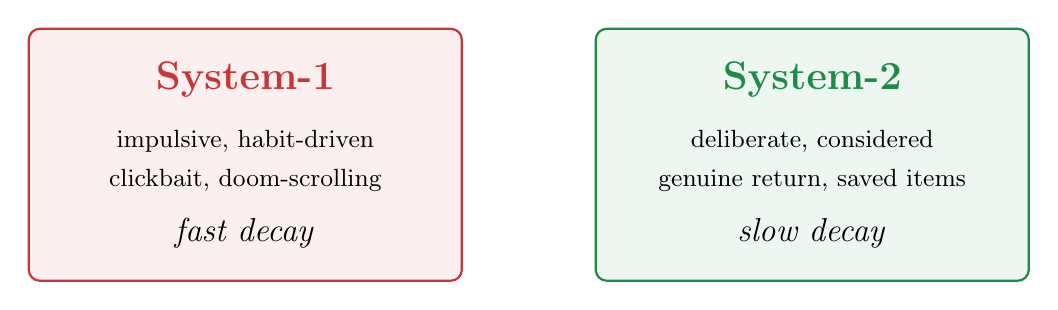
\begin{tikzpicture}[every node/.style={font=\large}]
    \node[draw=warn,thick,rounded corners,minimum width=5.5cm,minimum height=3.2cm,
          align=center,fill=warn!8] (s1) at (-3.6,0)
      {\textbf{\textcolor{warn}{\Large System-1}}\\[0.25cm]
       \small impulsive, habit-driven\\
       \small clickbait, doom-scrolling\\[0.2cm]
       \emph{fast decay}};
    \node[draw=good,thick,rounded corners,minimum width=5.5cm,minimum height=3.2cm,
          align=center,fill=good!8] (s2) at (3.6,0)
      {\textbf{\textcolor{good}{\Large System-2}}\\[0.25cm]
       \small deliberate, considered\\
       \small genuine return, saved items\\[0.2cm]
       \emph{slow decay}};
  \end{tikzpicture}

  \vspace{0.7cm}
  \begin{center}
    \large \textcolor{soft}{Engagement signals lump them together.}\\[0.2cm]
    \large{\bfseries\textcolor{accent}{We want to pull them apart from data.}}
  \end{center}
\end{frame}

% =========================================================================
% Slide 3: Paper's model
\begin{frame}{The paper's idea: dual-kernel Hawkes process}
  \vspace{0.2cm}
  \centering
  Each past event leaves \emph{two} echoes in future arrival intensity.

  \vspace{0.3cm}
  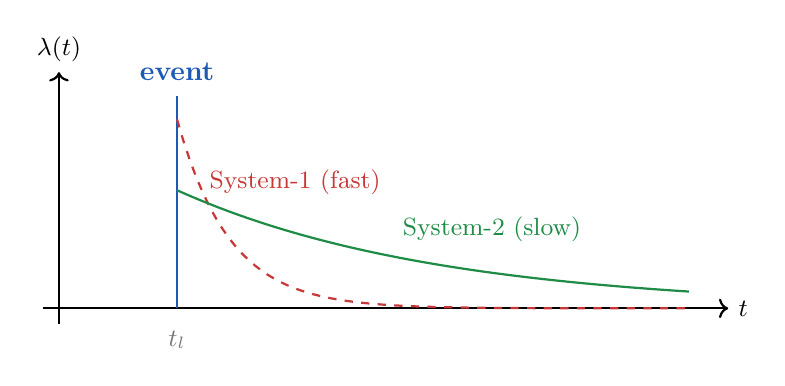
\begin{tikzpicture}[scale=1.0,every node/.style={font=\small}]
    \draw[->, thick] (-0.2,0) -- (8.5,0) node[right]{$t$};
    \draw[->, thick] (0,-0.2) -- (0,3) node[above]{$\lambda(t)$};

    \draw[accent, thick] (1.5,0) -- (1.5,2.7);
    \node[accent, font=\bfseries] at (1.5, 3.0) {event};

    \draw[warn, thick, dashed, domain=1.5:8, samples=80] plot (\x, {2.4*exp(-1.5*(\x-1.5))});
    \node[warn] at (3.0, 1.6) {\small System-1 (fast)};

    \draw[good, thick, domain=1.5:8, samples=80] plot (\x, {1.5*exp(-0.3*(\x-1.5))});
    \node[good] at (5.5, 1.0) {\small System-2 (slow)};

    \node[soft] at (1.5, -0.4) {\small $t_l$};
  \end{tikzpicture}

  \vspace{0.4cm}
  $$\lambda(t) \;=\; \mu \;+\; \sum_{t_l < t}
    \Big[\, \textcolor{warn}{\alpha^1\beta^1 e^{-\beta^1(t-t_l)}}
        \;+\; \textcolor{good}{\alpha^2\beta^2 e^{-\beta^2(t-t_l)}}\,\Big]$$
\end{frame}

% =========================================================================
% Slide 4: The paper's identifiability theorem
\begin{frame}{The paper's identifiability theorem}
  \vspace{0.4cm}

  \begin{center}
    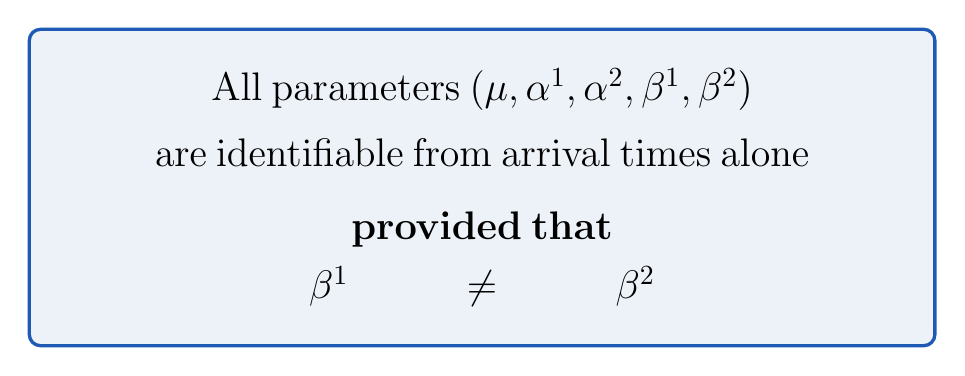
\begin{tikzpicture}
      \node[draw=accent, very thick, rounded corners, fill=accent!8,
            inner sep=0.5cm, text width=10.5cm, align=center]
      {\Large All parameters $(\mu, \alpha^1, \alpha^2, \beta^1, \beta^2)$\\[0.2cm]
       are identifiable from arrival times alone\\[0.3cm]
       \textbf{provided that}\\[0.2cm]
       \Large $\beta^1 \;\neq\; \beta^2$};
    \end{tikzpicture}
  \end{center}

  \vspace{0.5cm}

  \begin{itemize}
    \item Two distinct decays $\Rightarrow$ two distinguishable kernels.
    \item Inference works on \emph{just} the times $\{t_k\}$ --- no marks needed.
    \item \textcolor{soft}{Mixture-of-exponentials identifiability (Teicher 1961).}
  \end{itemize}

  \vspace{0.4cm}

  \centering\textcolor{accent}{\bfseries So far so good --- but what if the two timescales coincide?}
\end{frame}

% =========================================================================
% Slide 5: Where the paper breaks
\begin{frame}{Where it breaks}
  \vspace{0.3cm}
  \centering
  \begin{minipage}{0.45\textwidth}
    \centering
    \textbf{When $\beta^1 = \beta^2$:}\\[0.4cm]
    Two exponentials become indistinguishable.\\[0.4cm]
    \textcolor{warn}{\bfseries The kernels collide.}\\[0.3cm]
    Inference can no longer attribute past events to the right system.
  \end{minipage}\hfill
  \begin{minipage}{0.5\textwidth}
    \centering
    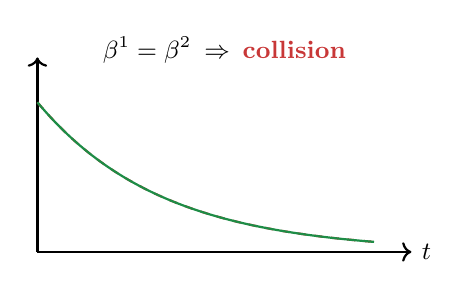
\begin{tikzpicture}[scale=0.95,every node/.style={font=\small}]
      \draw[->, thick] (0,0) -- (5,0) node[right]{$t$};
      \draw[->, thick] (0,0) -- (0,2.6);
      \draw[warn, thick, dashed, domain=0:4.5, samples=80] plot (\x, {2.0*exp(-0.6*\x)});
      \draw[good, thick, domain=0:4.5, samples=80] plot (\x, {2.0*exp(-0.6*\x)});
      \node at (2.5,2.7) {\small $\beta^1 = \beta^2$ \,$\Rightarrow$\, \textcolor{warn}{\bfseries collision}};
    \end{tikzpicture}
  \end{minipage}

  \vspace{0.7cm}
  \begin{center}
    \large \textcolor{accent}{\bfseries Real systems may have similar timescales.}\\[0.1cm]
    \textcolor{soft}{Identifiability shouldn't depend on a single fragile inequality.}
  \end{center}
\end{frame}

% =========================================================================
% Slide 6: Our hypothesis
\begin{frame}{Our hypothesis}
  \vspace{0.5cm}

  \begin{center}
    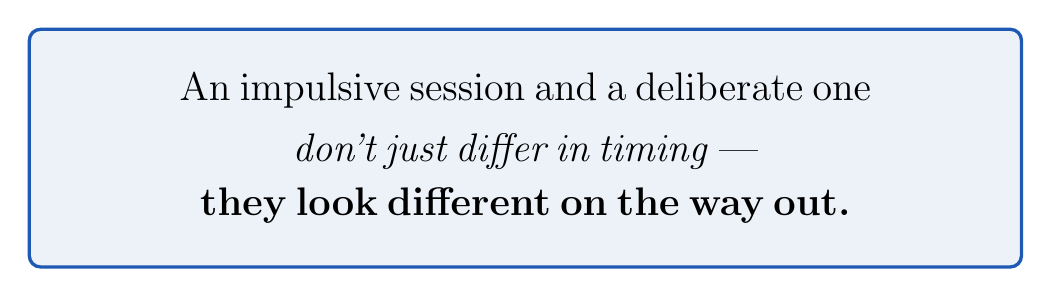
\begin{tikzpicture}
      \node[draw=accent, very thick, rounded corners, fill=accent!8,
            inner sep=0.55cm, text width=11.5cm, align=center]
      {\Large An impulsive session and a deliberate one\\[0.15cm]
       \emph{don't just differ in timing} ---\\[0.2cm]
       \Large \textbf{they look different on the way out.}};
    \end{tikzpicture}
  \end{center}

  \vspace{0.5cm}

  \begin{itemize}\setlength{\itemsep}{0.2cm}
    \item Each event leaves an \textbf{engagement mark}: clicks, dwell time, like flag.
    \item If marks differ across systems, they form a \emph{second} identifiability channel.
    \item \textcolor{accent}{\bfseries Either timing or marks should suffice --- we shouldn't need both.}
  \end{itemize}
\end{frame}

% =========================================================================
% Slide 7: Engagement marks defined
\begin{frame}{Engagement marks: what we observe per event}
  \vspace{0.2cm}

  \begin{center}
  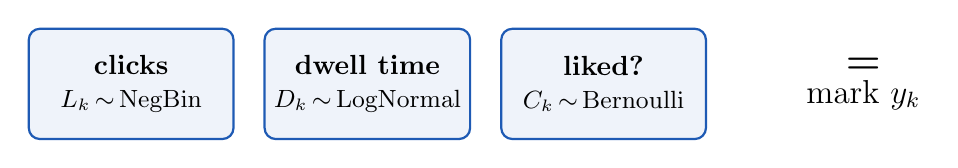
\begin{tikzpicture}[every node/.style={font=\normalsize}]
    \node[draw=accent,thick,rounded corners,minimum width=2.6cm,minimum height=1.4cm,
          fill=accent!7,align=center] (a) at (-4.3,0)
      {\textbf{clicks}\\\small $L_k$\,$\sim$\,NegBin};
    \node[draw=accent,thick,rounded corners,minimum width=2.6cm,minimum height=1.4cm,
          fill=accent!7,align=center] (b) at (-1.3,0)
      {\textbf{dwell time}\\\small $D_k$\,$\sim$\,LogNormal};
    \node[draw=accent,thick,rounded corners,minimum width=2.6cm,minimum height=1.4cm,
          fill=accent!7,align=center] (c) at (1.7,0)
      {\textbf{liked?}\\\small $C_k$\,$\sim$\,Bernoulli};
    \node[align=center] at (5.0,0) {\Large \textbf{=}\\[-0.05cm] \large mark $y_k$};
  \end{tikzpicture}
  \end{center}

  \vspace{0.5cm}

  \begin{center}
    \begin{tabular}{@{}lcc@{}}
      \toprule
       & \textcolor{warn}{System-1 session} & \textcolor{good}{System-2 session}\\
      \midrule
      clicks & $\sim 3$ & $\sim 12$ \\
      dwell  & $\sim 1$ unit & $\sim 5$ units \\
      liked  & 5\%   & 60\% \\
      \bottomrule
    \end{tabular}
  \end{center}

  \vspace{0.4cm}
  \centering
  \textcolor{soft}{\small Mixed-type product: each component is identifiable on its own (Teicher 1961, 1963).}
\end{frame}

% =========================================================================
% Slide 8: The marked model
\begin{frame}{The marked model}
  \vspace{0.2cm}

  \textbf{1. Arrival times} (unchanged from the paper):
  $$\lambda(t) = \mu + \sum_{t_l < t}
    \Big[\alpha^1\beta^1 e^{-\beta^1(t-t_l)} + \alpha^2\beta^2 e^{-\beta^2(t-t_l)}\Big]$$

  \vspace{0.2cm}

  \textbf{2. Each event} carries a latent system label $z_k \in \{1,2\}$ and a mark:
  $$y_k \mid z_k = j \;\sim\; F_j(\,\cdot\,;\theta_j)$$
  $$F_j \;=\; \mathrm{NegBin}(\lambda_j, r_j) \;\otimes\; \mathrm{LogNormal}(m_j, \sigma_j^2) \;\otimes\; \mathrm{Bernoulli}(p_j)$$

  \vspace{0.4cm}

  \begin{center}
    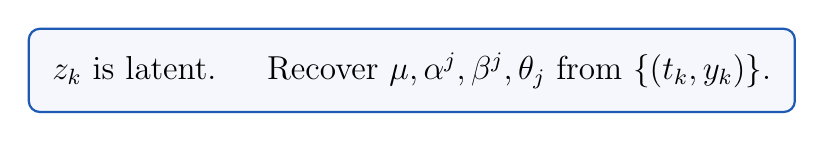
\begin{tikzpicture}
      \node[draw=accent, thick, rounded corners, fill=lightbg, inner sep=0.3cm]
      {\large $z_k$ is latent.\;\;\;\; Recover $\mu, \alpha^j, \beta^j, \theta_j$ from $\{(t_k, y_k)\}$.};
    \end{tikzpicture}
  \end{center}
\end{frame}

% =========================================================================
% Slide 9: Our theorem
\begin{frame}{Our theorem}
  \vspace{0.6cm}
  \begin{center}
    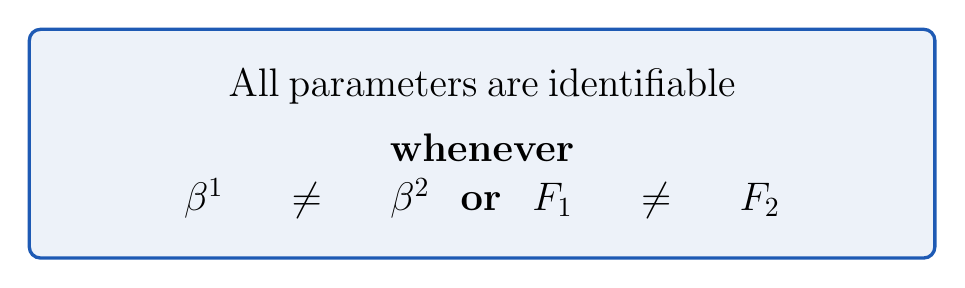
\begin{tikzpicture}
      \node[draw=accent, very thick, rounded corners, fill=accent!8,
            inner sep=0.5cm, text width=10.5cm, align=center]
      {\Large All parameters are identifiable\\[0.2cm]
       \textbf{whenever}\\[0.2cm]
       \Large $\beta^1 \;\neq\; \beta^2$ \;\;\textbf{or}\;\; $F_1 \;\neq\; F_2$};
    \end{tikzpicture}
  \end{center}

  \vspace{0.6cm}

  \begin{itemize}
    \item Either channel \emph{alone} suffices.
    \item \textbf{Failure mode:} both channels collapse simultaneously.
    \item \textbf{Strictly stronger} than the paper's result, which needs the timing channel only.
  \end{itemize}
\end{frame}

% =========================================================================
% Slide 10: Proof sketch
\begin{frame}{Proof sketch in three steps}
  \vspace{0.6cm}
  \centering
  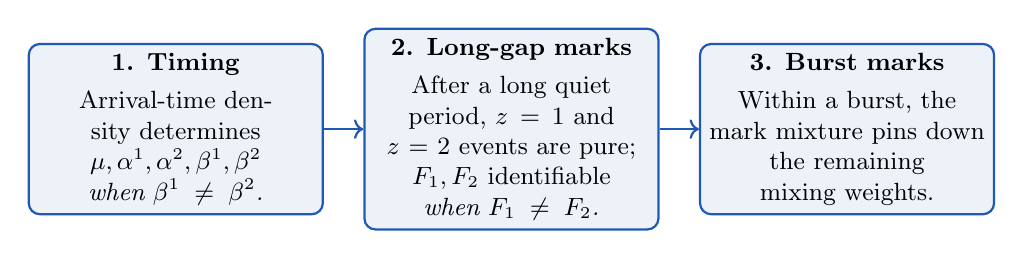
\begin{tikzpicture}[node distance=0.5cm,every node/.style={font=\small}]
    \node[draw=accent,thick,rounded corners,fill=accent!8,minimum height=2cm,
          text width=3.5cm,align=center] (a)
      {\textbf{1. Timing}\\[0.1cm]
       Arrival-time density determines\\
       $\mu, \alpha^1, \alpha^2, \beta^1, \beta^2$\\
       \emph{when $\beta^1 \neq \beta^2$.}};
    \node[draw=accent,thick,rounded corners,fill=accent!8,minimum height=2cm,
          text width=3.5cm,align=center, right=of a] (b)
      {\textbf{2. Long-gap marks}\\[0.1cm]
       After a long quiet period, $z = 1$ and $z = 2$ events are pure;\\
       $F_1, F_2$ identifiable\\
       \emph{when $F_1 \neq F_2$.}};
    \node[draw=accent,thick,rounded corners,fill=accent!8,minimum height=2cm,
          text width=3.5cm,align=center, right=of b] (c)
      {\textbf{3. Burst marks}\\[0.1cm]
       Within a burst, the mark mixture pins down\\
       the remaining mixing weights.};
    \draw[->, thick, accent] (a) -- (b);
    \draw[->, thick, accent] (b) -- (c);
  \end{tikzpicture}

  \vspace{0.6cm}

  \begin{center}
    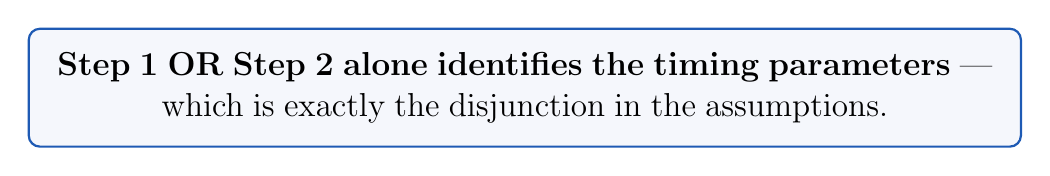
\begin{tikzpicture}
      \node[draw=accent, thick, rounded corners, fill=lightbg, inner sep=0.3cm,
            text width=12cm, align=center]
      {\large \textbf{Step 1 OR Step 2 alone identifies the timing parameters} ---\\[0.1cm]
       which is exactly the disjunction in the assumptions.};
    \end{tikzpicture}
  \end{center}
\end{frame}

% =========================================================================
% Slide 11: Inference --- branching latent structure
\begin{frame}{Inference: every event has a hidden source}
  \vspace{0.3cm}
  \centering
  For event $k$, the latent ``source'' is one of:

  \vspace{0.4cm}

  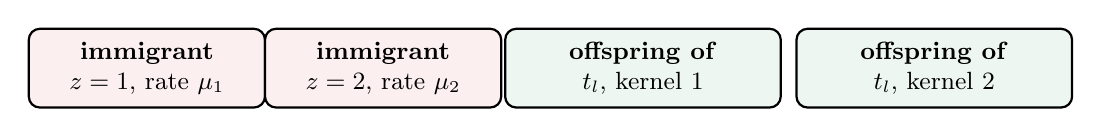
\begin{tikzpicture}[every node/.style={font=\small}]
    \node[draw,thick,rounded corners,fill=warn!8,minimum width=3.0cm,minimum height=1.0cm,align=center] (i1) at (-4.5,0)
      {\textbf{immigrant}\\$z = 1$, rate $\mu_1$};
    \node[draw,thick,rounded corners,fill=warn!8,minimum width=3.0cm,minimum height=1.0cm,align=center] (i2) at (-1.5,0)
      {\textbf{immigrant}\\$z = 2$, rate $\mu_2$};
    \node[draw,thick,rounded corners,fill=good!8,minimum width=3.5cm,minimum height=1.0cm,align=center] (o1) at (1.8,0)
      {\textbf{offspring of}\\$t_l$, kernel $1$};
    \node[draw,thick,rounded corners,fill=good!8,minimum width=3.5cm,minimum height=1.0cm,align=center] (o2) at (5.5,0)
      {\textbf{offspring of}\\$t_l$, kernel $2$};
  \end{tikzpicture}

  \vspace{0.5cm}

  \begin{itemize}
    \item Sum over $l < k$: at most $\sim 4N$ candidate sources for a sequence of length $N$.
    \item Posterior over sources gives every parameter as a weighted MLE.
    \item Two-step EM: assign sources (E), update parameters (M).
  \end{itemize}
\end{frame}

% =========================================================================
% Slide 12: E-step
\begin{frame}{E-step --- closed form}
  \vspace{0.6cm}

  Posterior responsibility of each candidate source for event $k$:

  \vspace{0.3cm}

  $$r_{k,\mathrm{imm},j} \;\propto\; \mu_j \cdot F_j(y_k;\theta_j)$$

  \vspace{0.2cm}

  $$r_{k,l,j} \;\propto\; \underbrace{\alpha^j\beta^j e^{-\beta^j(t_k - t_l)}}_{\textcolor{soft}{\text{timing contribution}}}
                          \;\times\; \underbrace{F_j(y_k;\theta_j)}_{\textcolor{soft}{\text{mark density}}}$$

  \vspace{0.5cm}

  \begin{itemize}
    \item Normalise row-wise so each event's source distribution sums to 1.
    \item Computed in log-space for numerical stability.
    \item \textbf{Both timing and marks enter the responsibility} --- this is where the second channel does work.
  \end{itemize}
\end{frame}

% =========================================================================
% Slide 13: M-step
\begin{frame}{M-step --- closed form}
  \vspace{0.4cm}

  Each parameter is a weighted average using the responsibilities $r_{k,\cdot,j}$:

  \vspace{0.2cm}

  $$\mu_j \leftarrow \frac{\sum_k r_{k,\mathrm{imm},j}}{T}, \qquad
    \alpha^j \leftarrow \frac{\sum_{k,l} r_{k,l,j}}{N}$$

  $$\beta^j \leftarrow \frac{\sum_{k,l} r_{k,l,j}}{\sum_{k,l} r_{k,l,j}\,(t_k - t_l)}, \qquad
    \theta_j \leftarrow \text{weighted MLE on } \{y_k\}$$

  \vspace{0.5cm}

  \begin{itemize}
    \item Anchor $\beta^1 > \beta^2$ via post-step swap to avoid label-degeneracy.
    \item Multi-restart wrapper for the genuinely flat regime ($s = 0$ in Exp 4).
    \item \textbf{No gradient descent anywhere.}
  \end{itemize}
\end{frame}

% =========================================================================
% Slide 14: Synthetic data setup
\begin{frame}{Synthetic data setup}
  \vspace{0.3cm}

  \begin{columns}[T,onlytextwidth]
    \column{0.48\textwidth}
      \textbf{Default ground truth}
      \begin{itemize}\setlength{\itemsep}{0.05cm}
        \item $\mu_1 = 0.05,\;\mu_2 = 0.03$
        \item $\alpha^1 = 0.4,\;\alpha^2 = 0.3$
        \item $\beta^1 = 1.0,\;\beta^2 = 0.1$
        \item Mark separation: $\sim 4\times$ in clicks, $\sim 5\times$ in dwell
      \end{itemize}

    \column{0.48\textwidth}
      \textbf{Pipeline}
      \begin{itemize}\setlength{\itemsep}{0.05cm}
        \item Ogata thinning simulator
        \item Ground-truth $z_k$ recorded
        \item Branching-EM, 100--150 iters
        \item 4--5 random seeds per setting
      \end{itemize}
  \end{columns}

  \vspace{0.5cm}

  \begin{center}
    
\begin{tikzpicture}
      \node[draw=accent, thick, rounded corners, fill=accent!8, inner sep=0.3cm, text width=11.5cm, align=center]
      {\textbf{Each experiment varies one axis} on top of this default --- horizon $T$, gap $\beta^1 - \beta^2$, or mark separation $s$.};
    \end{tikzpicture}
  \end{center}
\end{frame}

% =========================================================================
% Slide 15: Experiment 1
\begin{frame}{Experiment 1 --- Consistency}
  \vspace{0.1cm}
  \begin{center}
    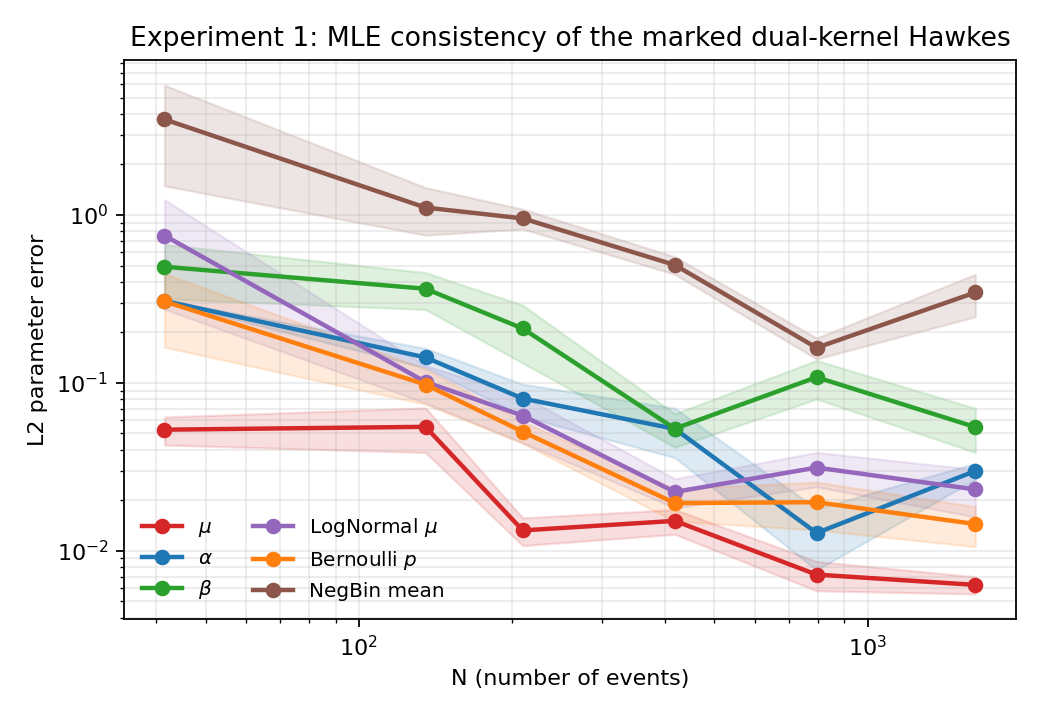
\includegraphics[width=0.62\textwidth]{exp1_consistency.png}
  \end{center}

  \vspace{-0.1cm}
  \begin{itemize}
    \item Sweep horizon $T$ across roughly an order of magnitude.
    \item Every parameter's L2 error decays toward zero as $N$ grows.
    \item Confirms that the marked-MLE is consistent --- the estimator works \emph{at all}.
  \end{itemize}
\end{frame}

% =========================================================================
% Slide 16: Experiment 2 --- headline
\begin{frame}{Experiment 2 --- Headline $\beta$-gap result}
  \vspace{0.1cm}
  \begin{center}
    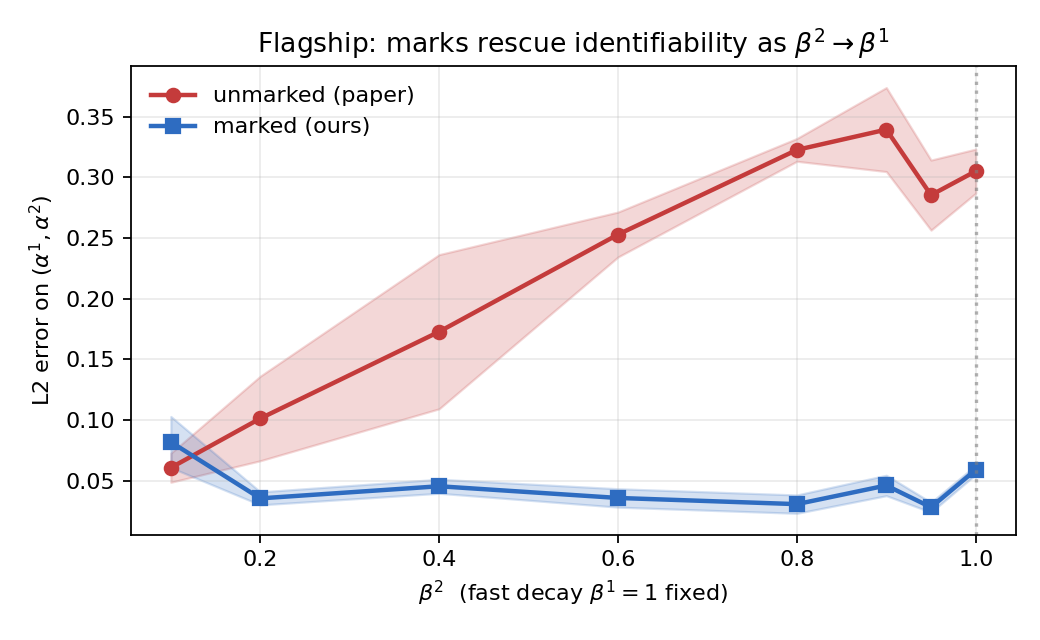
\includegraphics[width=0.72\textwidth]{exp2_beta_gap.png}
  \end{center}

  \vspace{-0.2cm}
  \begin{center}
    \begin{tabular}{ll}
      \textcolor{warn}{\textbf{Unmarked baseline}} & error climbs as $\beta^2 \to \beta^1$ \\
      \textcolor{good}{\textbf{Our marked model}}  & error stays flat at every gap \\
    \end{tabular}
  \end{center}

  \vspace{0.2cm}
  \centering\textcolor{accent}{\large\bfseries 5.2$\times$ lower error at the failure regime $\beta^1 = \beta^2 = 1$.}
\end{frame}

% =========================================================================
% Slide 17: Experiment 3
\begin{frame}{Experiment 3 --- Sample complexity at moderate gap}
  \vspace{0.1cm}
  \begin{center}
    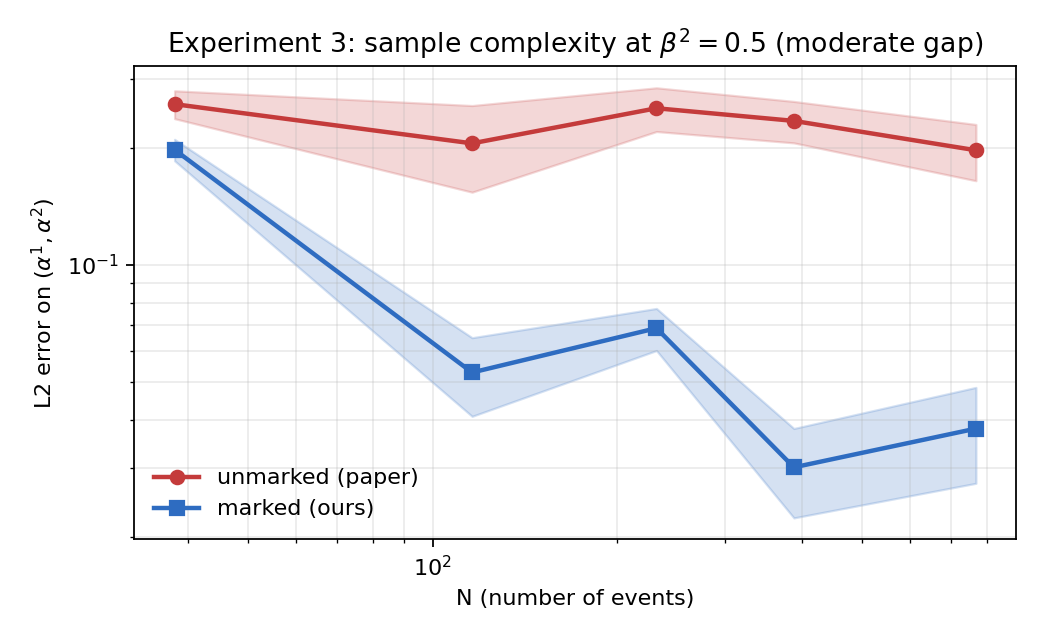
\includegraphics[width=0.62\textwidth]{exp3_sample_complexity.png}
  \end{center}

  \vspace{-0.1cm}
  \begin{itemize}
    \item Fix $\beta^1/\beta^2 = 2$ --- timing is technically identifiable.
    \item \textbf{Marks still help.} Marked beats unmarked at every horizon.
    \item Unmarked plateaus at error $\sim 0.32$; marked drops below 0.1 by $N \approx 120$.
  \end{itemize}
\end{frame}

% =========================================================================
% Slide 18: Experiment 4
\begin{frame}{Experiment 4 --- Failure-mode test}
  \vspace{0.1cm}
  \begin{center}
    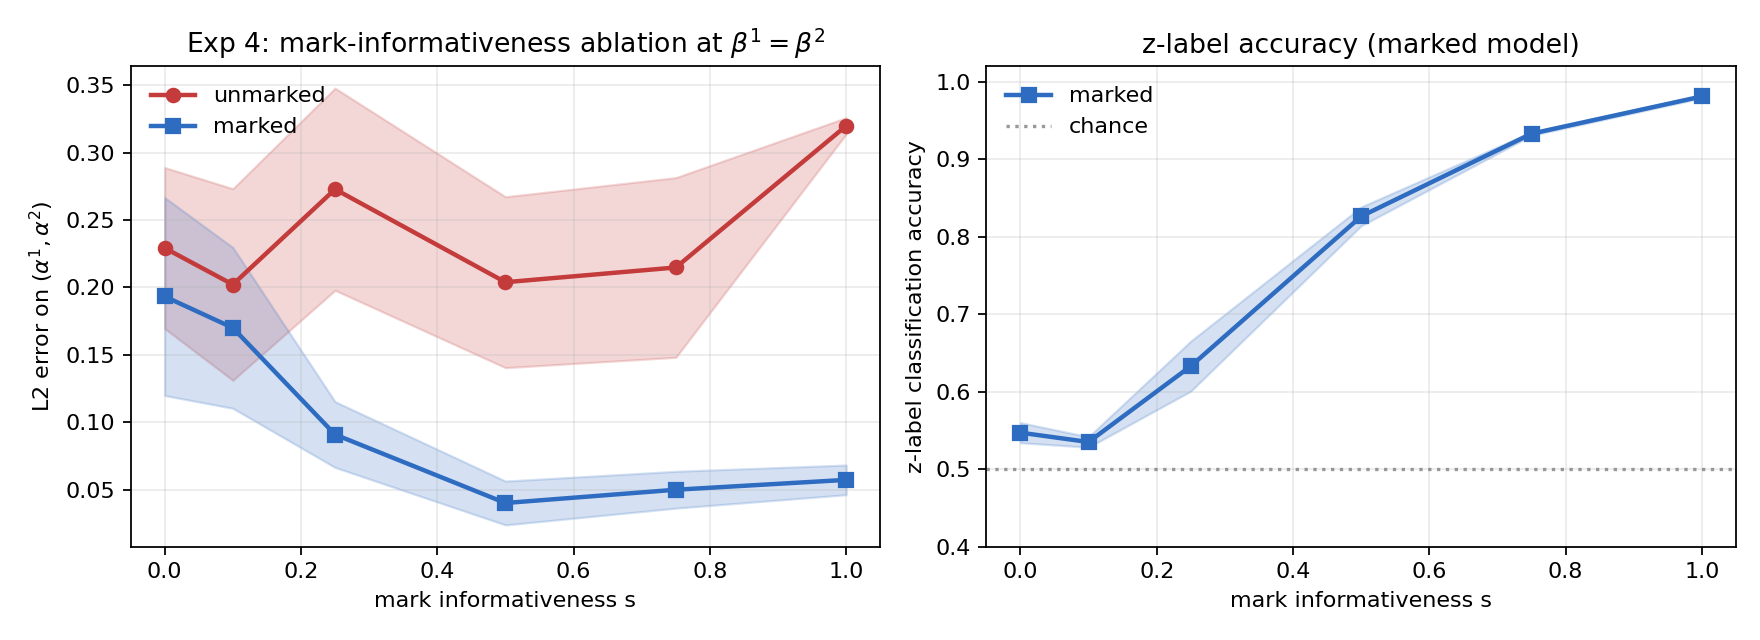
\includegraphics[width=0.72\textwidth]{exp4_mark_informativeness.png}
  \end{center}

  \vspace{-0.2cm}
  Force $\beta^1 = \beta^2$ (timing channel dead). Slide mark separation $s$ from 0 to 1.

  \vspace{0.15cm}
  \begin{itemize}
    \item $s = 0$: both channels dead $\Rightarrow$ $z$-accuracy at chance (54.7\%).
    \item $s = 1$: marks fully separate $\Rightarrow$ near-perfect recovery (98.1\% $z$-accuracy).
    \item Smooth ramp confirms the failure-mode corollary exactly.
  \end{itemize}
\end{frame}

% =========================================================================
% Slide 19a: Experiment 5 (held-out forecasting)
\begin{frame}{Experiment 5 --- Held-out forecasting}
  \vspace{0.05cm}
  \begin{center}
    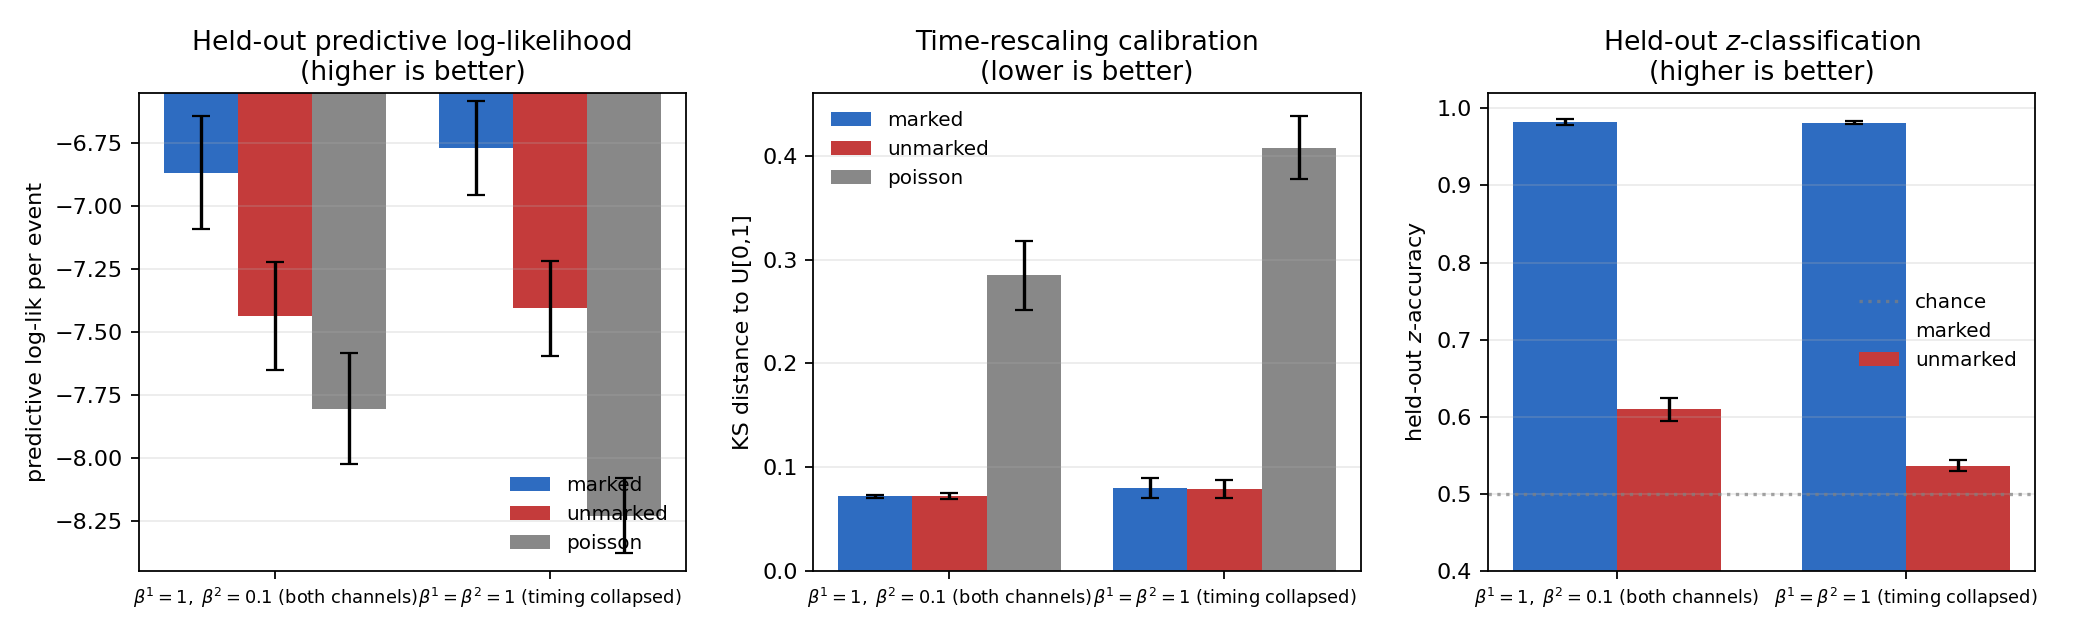
\includegraphics[width=0.78\textwidth]{exp5_forecasting.png}
  \end{center}

  \vspace{-0.15cm}
  Train on 70\% of a sequence; evaluate predictions on the held-out 30\%.

  \vspace{0.1cm}
  \begin{itemize}
    \item Marked beats unmarked by $\sim$\textbf{0.6 nats/event} in joint predictive log-lik (both regimes).
    \item Time-rescaling calibration: marked $\approx$ unmarked $\ll$ Poisson --- Hawkes structure matters.
    \item Held-out $z$-accuracy: marked \textbf{98\%} vs unmarked \textbf{54\%} (chance) at $\beta^1 = \beta^2$.
  \end{itemize}
\end{frame}

% =========================================================================
% Slide 20: Summary + bottom line
\begin{frame}{Bottom line}
  \vspace{0.0cm}
  \begin{center}
    \begin{tabular}{@{}p{2.8cm}p{4.5cm}p{6.0cm}@{}}
      \toprule
      \textbf{Experiment} & \textbf{Tests} & \textbf{Says} \\
      \midrule
      1.\ Consistency        & MLE consistency        & The estimator works at all. \\[0.1cm]
      2.\ $\beta$-gap        & Marks rescue collapse  & Theorem strictly stronger than paper's. \\[0.1cm]
      3.\ Sample complexity  & Finite-sample gain     & Advantage holds in realistic regimes. \\[0.1cm]
      4.\ Informativeness    & Failure-mode corollary & Both channels can't fail at once. \\[0.1cm]
      5.\ Forecasting        & In-sample $\Rightarrow$ out-of-sample & Better recovery $\Rightarrow$ better held-out predictions. \\
      \bottomrule
    \end{tabular}
  \end{center}

  \vspace{0.5cm}

  \begin{center}
    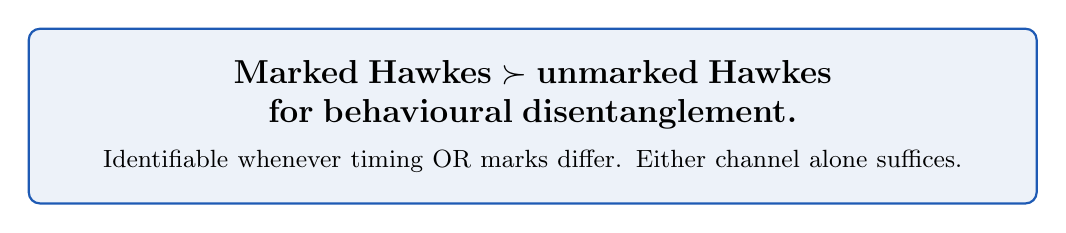
\begin{tikzpicture}
      \node[draw=accent, thick, rounded corners, fill=accent!8, inner sep=0.4cm,
            text width=12cm, align=center]
      {\large \textbf{Marked Hawkes $\succ$ unmarked Hawkes for behavioural disentanglement.}\\[0.15cm]
       \small Identifiable whenever timing OR marks differ. Either channel alone suffices.};
    \end{tikzpicture}
  \end{center}
\end{frame}

% =========================================================================
% Slide 21: Thank you
\begin{frame}[plain]
  \begin{center}
    \vspace{2cm}
    {\Huge\bfseries\textcolor{accent}{Thank you}}\\[1cm]
    {\Large Questions?}\\[2cm]
    
\begin{tikzpicture}\draw[accent,thick] (-3,0) -- (3,0);\end{tikzpicture}\\[0.5cm]
    {\large Source paper: arXiv:2406.01611}
  \end{center}
\end{frame}

\end{document}
